\documentclass[letterpaper,11pt]{article}

\usepackage{latexsym}
\usepackage[empty]{fullpage}
\usepackage{titlesec}
\usepackage{marvosym}
\usepackage[usenames,dvipsnames]{color}
\usepackage{verbatim}
\usepackage{enumitem}
\usepackage[hidelinks]{hyperref}
\usepackage{fancyhdr}
\usepackage[english]{babel}
\usepackage{tabularx}
\usepackage{fontawesome5}
\usepackage{multicol}
\setlength{\multicolsep}{-3.0pt}
\setlength{\columnsep}{-1pt}
\input{glyphtounicode}

%new packages

\usepackage{fontenc}
\usepackage{amsmath}
\usepackage{amssymb}
\usepackage{graphicx}



%----------FONT OPTIONS----------

\pagestyle{fancy}
\fancyhf{} % clear all header and footer fields
\fancyfoot{}
\renewcommand{\headrulewidth}{0pt}
\renewcommand{\footrulewidth}{0pt}

% Adjust margins
\addtolength{\oddsidemargin}{-0.6in}
\addtolength{\evensidemargin}{-0.5in}
\addtolength{\textwidth}{1.19in}
\addtolength{\topmargin}{-.7in}
\addtolength{\textheight}{1.4in}

\urlstyle{same}

\raggedbottom
\raggedright
\setlength{\tabcolsep}{0in}

% Sections formatting
\titleformat{\section}{
  \vspace{-4pt}\scshape\raggedright\large\bfseries
}{}{0em}{}[\color{black}\titlerule \vspace{-5pt}]



% Ensure that generate pdf is machine readable/ATS parsable
\pdfgentounicode=1

%-------------------------
% Custom commands
\newcommand{\resumeItem}[1]{
  \item\small{
    {#1 \vspace{-2pt}}
  }
}

\newcommand{\classesList}[4]{
    \item\small{
        {#1 #2 #3 #4 \vspace{-2pt}}
  }
}

\newcommand{\resumeSubheading}[4]{
  \vspace{-2pt}\item
    \begin{tabular*}{1.0\textwidth}[t]{l@{\extracolsep{\fill}}r}
      \textbf{#1} & \textbf{\small #2} \\
      \textit{\small#3} & \textit{\small #4} \\
    \end{tabular*}\vspace{-7pt}
}

\newcommand{\resumeSubSubheading}[2]{
    \item
    \begin{tabular*}{0.97\textwidth}{l@{\extracolsep{\fill}}r}
      \textit{\small#1} & \textit{\small #2} \\
    \end{tabular*}\vspace{-7pt}
}

\newcommand{\resumeProjectHeading}[2]{
    \item
    \begin{tabular*}{1.001\textwidth}{l@{\extracolsep{\fill}}r}
      \small#1 & \textbf{\small #2}\\
    \end{tabular*}\vspace{-7pt}
}


\newcommand{\resumeSubItem}[1]{\resumeItem{#1}\vspace{-4pt}}

\renewcommand\labelitemi{$\vcenter{\hbox{\tiny$\bullet$}}$}
\renewcommand\labelitemii{$\vcenter{\hbox{\tiny$\bullet$}}$}

\newcommand{\resumeSubHeadingListStart}{\begin{itemize}[leftmargin=0.0in, label={}]}
\newcommand{\resumeSubHeadingListEnd}{\end{itemize}}
\newcommand{\resumeItemListStart}{\begin{itemize}}
\newcommand{\resumeItemListEnd}{\end{itemize}\vspace{-5pt}}


\begin{document}
\fontfamily{cmr}\selectfont
\begin{center}
\parbox{3.0cm}{%
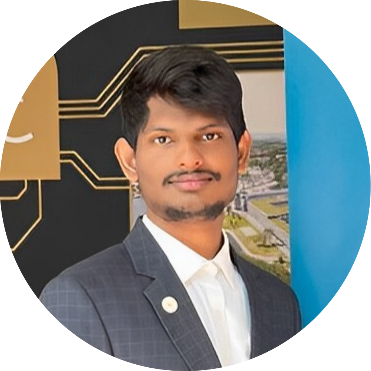
\includegraphics[width=2.7cm,clip]{images/resume_pic_m.png}}
\parbox{\dimexpr\linewidth-3.8cm\relax}{
\vspace{-20pt}
\begin{tabularx}{\linewidth}{L r} \\
    {\Huge \scshape  Venkata Sai Yakkshit Reddy Asodi}~
    \href{https://www.cedzlabs.com/yakkshit}{\vspace{1pt}}\\
      Berlin, Germany. \\ \vspace{1pt}
     \small \raisebox{-0.1\height}\faPhone\ +91 8179936156 ~ \href{mailto:saiyakkshit2001@gmail.com}{\raisebox{-0.2\height}\faEnvelope\  {saiyakkshit2001@gmail.com}} ~ 
    \href{https://linkedin.com/in/yakkshit/}{\raisebox{-0.2\height}\faLinkedin\ {yakkshit}}  ~
    \href{https://yakkshit.com/}{\raisebox{-0.2\height}\faGlobe\ {yakkshit.com}}  ~
    \href{https://github.com/yakkshit}{\raisebox{-0.2\height}\faGithub{ yakkshit}}
    \vspace{-8pt}
    
\end{tabularx}
}
\end{center}

\vspace{-23pt}

\section{Summary}
Dynamic Software Engineer with extensive experience in designing AI-powered platforms, focusing on performance optimization, data pipelines, and conversational AI. Skilled in fine-tuning LLMs, ensuring security, and working closely with stakeholders to translate business needs into technical solutions. Looking to leverage technical proficiency in Python, Docker, and MongoDB to solve complex problems and drive innovation.

\section{Technical Skills}
\begin{itemize}[leftmargin=0.15in, label={}]
\small{\item{
\textbf{Languages:} Python, JavaScript (ES6+), HTML5, CSS3, SQL \\
\textbf{Frameworks:} React, Next.js, Django, Express.js \\
\textbf{Tools:} Docker, Git, Azure, MongoDB, Redis, Hugging Face \\
\textbf{Cloud:} AWS, Azure \\
\textbf{APIs:} RESTful, GraphQL, OpenAI API, Twilio, Stripe \\
\textbf{Data:} Redis, MongoDB, SQL, Firebase, Supabase \\
}}
\end{itemize}

\vspace{-7pt}
\section{Experience}

\resumeSubHeadingListStart

\resumeSubheading
{Circleup AG}{January 2024 -- Present}
{Lead Full Stack Engineer (Frontend Focus)}{Zurich, Switzerland}
\begin{itemize}
    \item Developed AI-driven conversational tools, ensuring seamless integration between LLM-powered backend and frontend interfaces, improving performance by 20\%.
    \item Optimized user experience by introducing modern UI components, leveraging React and Next.js for scalable solutions in fast-paced environments.
    \item Built scalable data pipelines using MongoDB and Redis to ensure real-time data availability and reduced latency.
\end{itemize}

\resumeSubheading
{Cedzlabs}{March 2023 -- January 2024}
{Full Stack Developer}{Remote, India}
\begin{itemize}
    \item Led the development of AI-assisted event scheduling platforms, using Python for backend APIs and React for user-friendly UIs.
    \item Integrated third-party services such as Google Calendar and Twilio for automated event management solutions.
\end{itemize}

\resumeSubHeadingListEnd

\section{Projects}

\resumeSubHeadingListStart

\resumeProjectHeading
{\textbf{AI-Powered Roleplay System} $|$ \emph{Docker, Azure, LLMs, Hugging Face}}{June 2023}
\begin{itemize}
    \item Designed an AI-based roleplay platform for customer support teams to practice and improve real-time interactions with customers.
    \item Fine-tuned large language models on Hugging Face to simulate human-like conversations with up to 90\% accuracy in natural language understanding.
\end{itemize}

\resumeProjectHeading
{\textbf{AI Resume Tuner} $|$ \emph{Next.js, Azure Cloud, RAG, LLMs}}{August 2023}
\begin{itemize}
    \item Developed a resume tuning application, utilizing Retrieval-Augmented Generation (RAG) and LLMs to customize resumes based on job descriptions.
    \item Deployed the backend on Azure Cloud ensuring secure and scalable performance.
\end{itemize}

\resumeSubHeadingListEnd

\section{Achievements \& Contributions}
\begin{itemize}[leftmargin=0.15in, label={}]
    \item Improved data pipeline performance by 25\% at Circleup, reducing latency for real-time data synchronization.
    \item Contributed to open-source AI research projects related to role-based conversational systems.
    \item Received performance-based recognition for delivering optimized, scalable code solutions in fast-paced environments.
\end{itemize}

\section{Languages}
\begin{itemize}
    \item Telugu - Native, English - Fluent, Hindi - Fluent, German - Elementary, Swedish - Elementary.
\end{itemize}

\end{document}